\section{Constructing the Clean Grounding Comparisons}
\label{app:construction}

A point should follow the requested object when either the query or the
object's position changes. The clean two-view construction makes this
requirement explicit. Four repaired source pairs contain a bottle, clock, cup,
and a bag annotated as backpack (Figure~\ref{fig:app-clean}). We retain the
annotation names in the queries. Cyclic pairing of distinct categories produces
four boards. For each board, both categories are queried and both left/right
arrangements are evaluated, giving $4\times2\times2=16$ paired queries per
intervention and model.

Each source view keeps its original size. A 16-pixel gray gutter separates the
two views on a canvas of size $(2W+16)\times H$. The target box is translated
by the panel offset; its shape is unchanged. Boxes are evaluation annotations
and never appear in model inputs. The image center lies in the gutter, so a
constant center response cannot solve this task.

\subsection{Queries and image regions}
Category prompts ask for the named object's location. Action prompts place the
same category in an interaction description and request that object's location.
Both ask for a single point in normalized 0--1000 coordinates over the entire
canvas. The action variant tests action-framed object localization; it does
not annotate a separate contact point on the object.

For target-window replacement, pixels inside the projected target rectangle
come from the converted view, while the remaining target view and the distractor
view remain original. Context replacement keeps that rectangle original and
converts the rest of the canvas, including the distractor view. Full conversion
uses converted versions of both views. The rectangle uses floor/ceiling integer
bounds and includes any background within the bounding box. This makes the
intervention an exact image-region crossover rather than a segmentation mask.

\subsection{Source correspondence}
The source manifest records pair IDs, camera-derived boxes, image digests, and
the composition recipe. The four clean pairs were selected from repaired
captures with recorded material-resolution checks. The earlier raster archive
contains 80 paired views of 16 targets, including a 30-pair close-view subset
of 12 targets. Some earlier original-MDL images contain material-resolution
errors. Those saved inputs support the readout analyses below; the clean window
experiment uses the repaired four-pair set. Query and position permutations
increase the tested comparisons without increasing the number of source objects.

\begin{figure}[p]
\centering
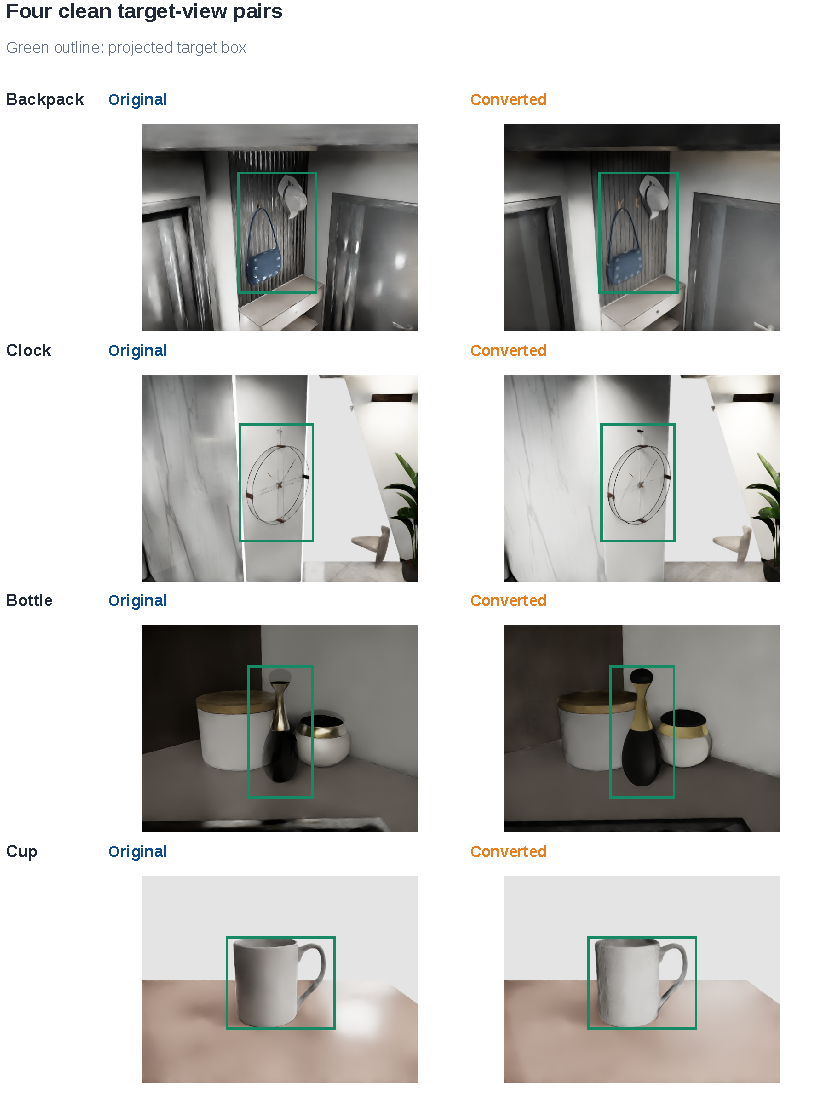
\includegraphics[width=\linewidth,height=.84\textheight,keepaspectratio]{appendix_clean_grounding.pdf}
\caption{The four repaired source pairs used to construct the clean two-view experiment. Boxes show the projected evaluation regions and are absent from model inputs. Both targets and both panel positions are queried on each composed board.}
\label{fig:app-clean}
\end{figure}
\FloatBarrier
